\chapter{Future work}
\label{chap:futurework}

In this chapter we discuss the improvements that can be done to our method in order to improve the solution.

\section{Improving the quality}

As we have seen the results section, catching the right effect balancing absorption and scattering requires a lot of tweaking of the parameters $M$ and $q$. This depends from the fact that an exponential sampling based on $\sigma_{tr}$ is not probably the best suited for the solution, thus providing good results. A further investigation of optimal sampling patterns would be required in order to obtain faithful results.

An idea we would like to explore is to use two separate disks with a different sampling radius, one accounting the absorption and one for the scattering contribution. The size of the radius of the two disk should be related to the scattering parameters, such as $\sigma_a$ and $\sigma_s$. Further investigation is required in this realm in order to obtain results applicable to a wide range of participating media.

Another direction we would like to explore is the automatic placing of the cameras. Because of the variety and possible concavity of meshes, it is very difficult to place cameras in a way to ensure the complete coverage of the object. The field in which to find ideas in order to fully cover the object would be 3D mesh acquisition using cameras. In this way, it will be possible for a user to avoid the tedious operation of placing the cameras in order to get a full coverage of the object. 

Another possibility in this area is to rotate the cameras during the rendering phase: in this case, fewer cameras will be necessary, but then an accumulation process would not be possible in the way we implemented it. It would require a great change to the way the algorithm works in order to get a solution.

\section{Improving the performance}
Regarding the implementation, we tought about some possible extensions in order to make the implementation faster and more reliable.

\begin{figure}[!h]
\centering
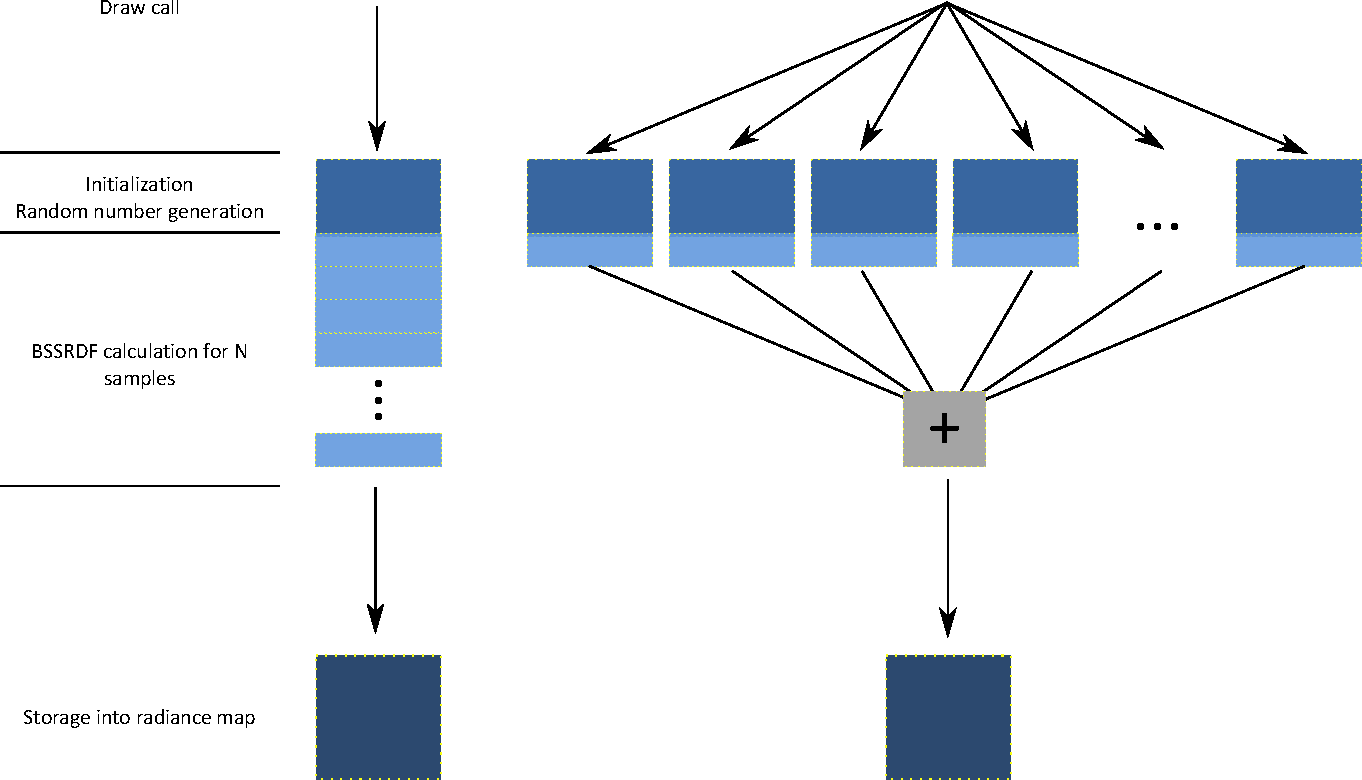
\includegraphics[width=0.7 \linewidth]{images/method/extension_shader.pdf}
\caption{Different approaches to rendering to the radiance map: on the left, our approach (one random number generation, multiple samples in the same shader invocation). On the right, the proposed approach: smaller shader invocations, that can be distributed on the GPU.}
\label{fig:shaderimprov}
\end{figure}

The first thing we have thought about would be to change the loop in step 2. The idea would be to have instead to have a single fragment shader invocation with cycling $N$ times on the samples, to have $N$ separate fragment shader invocations that calculate the result. The single invocations can be summed over using blending or atomic operations available since OpenGL 4.2. This would allow the GPU more flexibility in scheduling its work. However, we have seen in \ref{fig:shaderimprov} that also the random number generation is an expensive operation for the GPU, and that would have to be repeated for each of the $N$ fragments, potentially undermining the advantages of GPU scheduling. 

Another improvement in order to make the performance more reliable would be to make the cameras more adaptive. At the moment, the size of the light and directional cameras is fixed and set up by the user. A simple extension to the method would be to make the camera size adaptive, in order to adapt to the object bounding box. This would make the area in the radiance map texture space more consistent regarding to the size of the object, leading to a more predictable result. 

